\section{Introduction to Vehicle Dynamics}

To plan a feasible trajectory and to control the vehicle along it, we need to know how the vehicle reacts to the commands it receives. In this chapter we introduce the modeling problem, the terminology of vehicle dynamics, the forces generated by the tires and the main forces that act along the longitudinal direction.

\subsection{The modeling problem}
The objective of modeling is to derive a \textbf{mathematical object} that describes the behaviour of a system. It can be obtained in two ways: from the basic laws of physics, which is the approach followed in this course, or from input/output data.

In \textbf{physical modeling} we derive a set of equations from the physical laws that govern the system. A change in the system parameters is reflected directly in the model, and our knowledge of the system is used to give the model its structure. On the other hand, this knowledge is required, and some parameters can be difficult to measure or estimate.

In \textbf{data-driven modeling} we guess a state-space or black-box model, and we fit its parameters, which have no physical meaning, to the input/output data. A limited knowledge of the physics is less critical, and a well-established theory exists (\textbf{System Identification}). However, data are necessary, the experiments used to collect them must be carefully designed, and any change in the system requires repeating the entire modeling procedure.

\subsection{Terminology and notation}
Figure~\ref{fig:vehicle-notation} shows the main quantities used to describe a vehicle seen from above.

\begin{figure}[H]
    \centering
    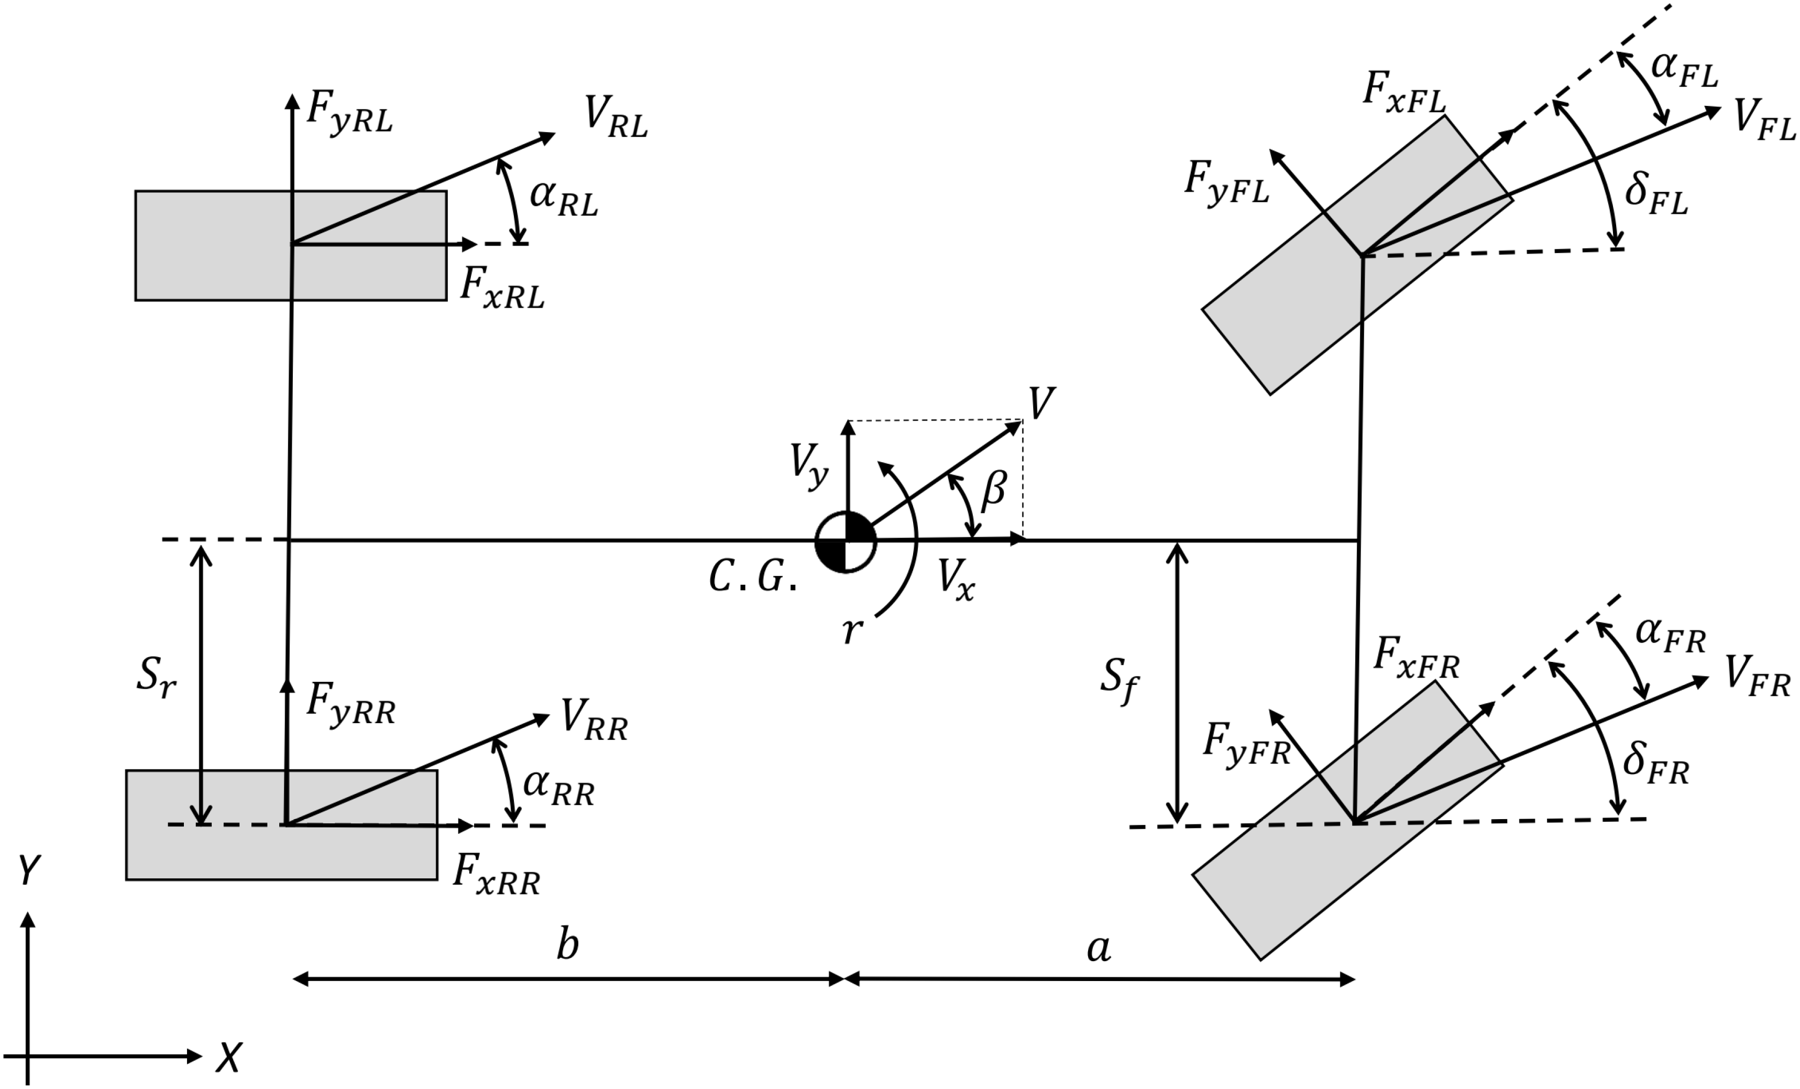
\includegraphics[width=0.72\textwidth]{images/C14_1.png}
    \caption{Vehicle quantities: velocities, tire forces, slip angles and steering angles of each wheel ($S_f$ and $S_r$ are half of the front and rear track)}
    \label{fig:vehicle-notation}
\end{figure}

\begin{table}[H]
    \centering
    \small
    \begin{tabular}[t]{ll}
        \hline
        \multicolumn{2}{l}{\textbf{Static parameters}}\\
        \hline
        $m$ & vehicle mass\\
        $l$ & vehicle length\\
        $a$ or $l_f$ & distance from CoG to front axle\\
        $b$ or $l_r$ & distance from CoG to rear axle\\
        $l_{wb}$ & wheelbase, $a + b$\\
        $I_z$ or $J_z$ & moment of inertia\\
        $g$ & gravitational acceleration\\
        \hline
        \multicolumn{2}{l}{\textbf{Pose in a global frame}}\\
        \hline
        $X$ & longitudinal position\\
        $Y$ & lateral position\\
        $\varphi$ & yaw or heading angle\\
        \hline
    \end{tabular}
    \hspace{0.6cm}
    \begin{tabular}[t]{ll}
        \hline
        \multicolumn{2}{l}{\textbf{Motion and forces}}\\
        \hline
        $\delta$ & steering angle\\
        $a_x$ & longitudinal acceleration\\
        $a_y$ & lateral acceleration\\
        $v_x$ & longitudinal velocity\\
        $v_y$ & lateral velocity\\
        $r$ & yaw rate (angular velocity)\\
        $F_x$ & longitudinal forces\\
        $F_y$ & lateral forces\\
        $F_z$ & vertical forces\\
        \hline
    \end{tabular}
    \caption{Notation used for the vehicle (CoG = centre of gravity)}
\end{table}

The \textbf{moment of inertia} $I_z$ is the ratio between the applied torque and the resulting angular acceleration about an axis. It represents how difficult it is to change the rotation rate around that axis:
\[
I_z = \frac{M_z}{\dot r}
\]

\subsubsection{Side slip angle}
A vehicle does not always move in the direction it is pointing. The \textbf{side slip angle} $\beta$ is the angle, at the CoG, between the direction of the velocity and the vehicle centerline. It depends on $v_x$ and $v_y$:
\[
\beta = \arctan\!\left(\frac{v_y}{v_x}\right)
\]

\begin{figure}[H]
    \centering
    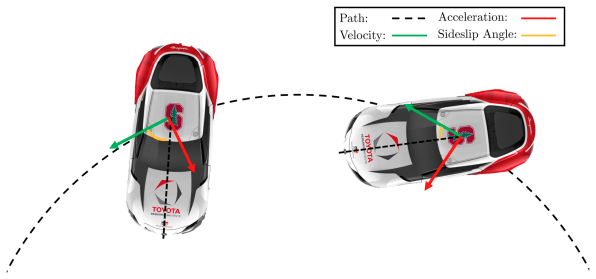
\includegraphics[width=0.55\textwidth]{images/C14_2.png}
    \caption{Velocity and acceleration of a vehicle for two different side slip angles}
\end{figure}

\subsubsection{Understeer and oversteer}
In \textbf{understeer} the front wheels lose traction and the car goes wide: it turns less than the steering angle requires, so there is less steering capacity. In \textbf{oversteer} the rear wheels lose traction and the rear of the car slides outwards: the car rotates more than expected, so there is more steering capacity than requested.

\begin{figure}[H]
    \centering
    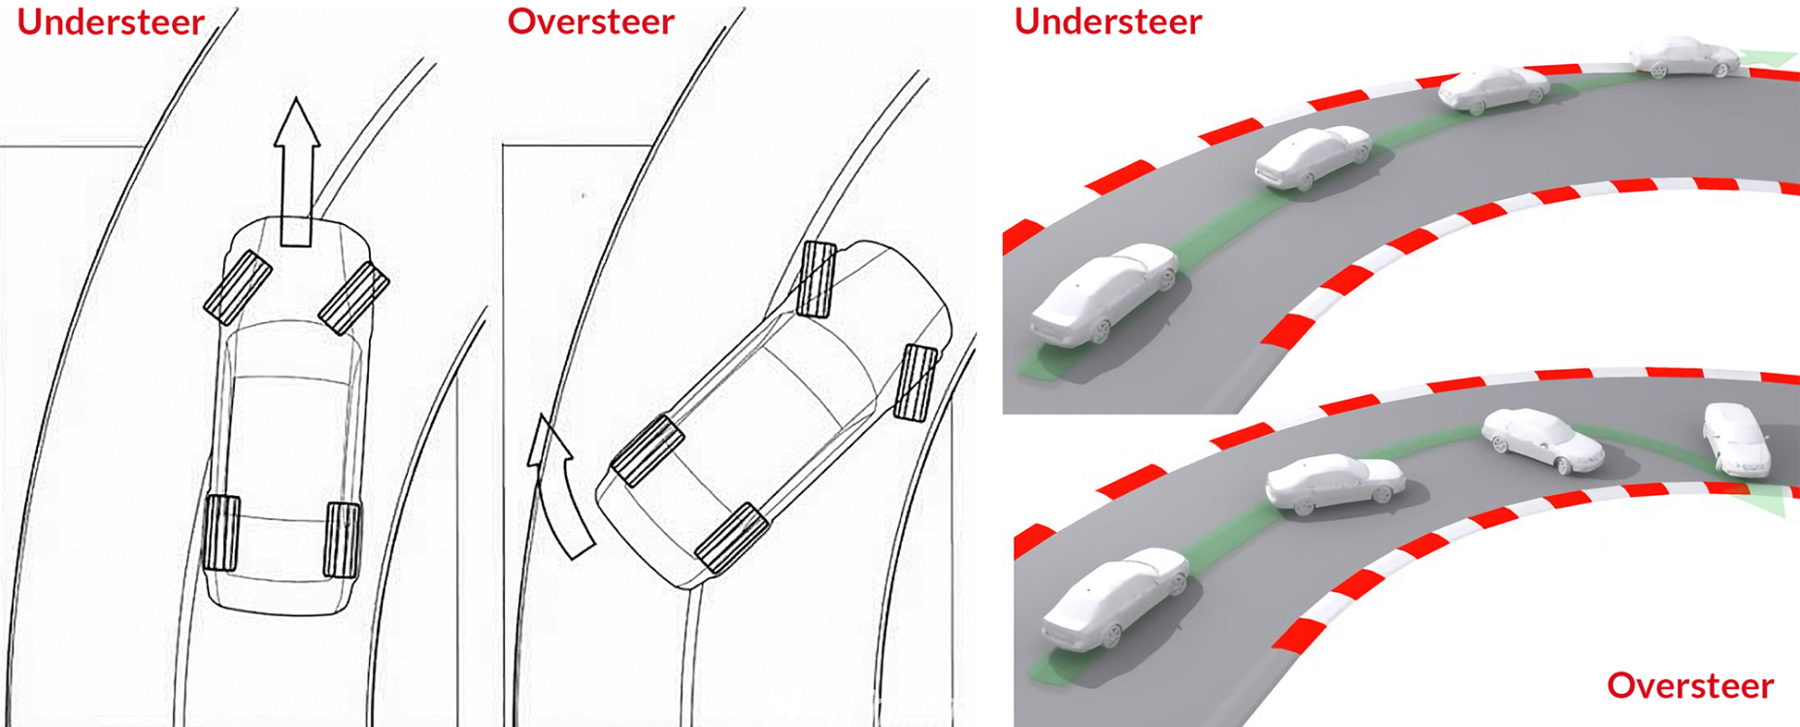
\includegraphics[width=0.55\textwidth]{images/C14_3.png}
    \caption{Understeer and oversteer}
\end{figure}

\subsubsection{Lateral slip angle}
\noindent\begin{minipage}[c]{0.74\textwidth}
A rolling tire that generates a lateral force deforms, so it does not travel exactly in the direction in which it points. The \textbf{lateral slip angle} $\alpha$ is the angle between the direction of travel of the tire and the tire centreline. For the front and rear axle it is:
\[
\alpha_f = -\arctan\!\left(\frac{v_y + r\, l_f}{v_x}\right) + \delta
\]
\[
\alpha_r = \arctan\!\left(-\frac{v_y - r\, l_r}{v_x}\right)
\]
The term $r\,l_f$ (or $-r\,l_r$) is the lateral velocity added at the axle by the rotation of the vehicle. Only the front axle steers, so only $\alpha_f$ contains $\delta$.
\end{minipage}\hfill
\begin{minipage}[c]{0.22\textwidth}
    \centering
    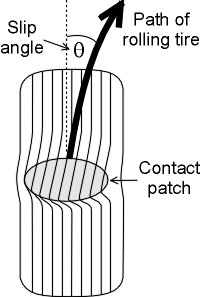
\includegraphics[width=\linewidth]{images/C14_4.png}
    \captionof{figure}{Slip angle of a rolling tire}
\end{minipage}

\subsubsection{Longitudinal slip}
The \textbf{longitudinal slip ratio} $\lambda$ compares the forward velocity of the tire with the velocity of its contact patch:
\[
\lambda = \frac{v_x - R\,\omega}{v_x}
\]
where $R$ is the rolling radius of the tire and $\omega$ the angular velocity of the wheel. With this definition $\lambda = 0$ is pure rolling, $\lambda > 0$ means that the wheel turns slower than the vehicle moves (braking), and $\lambda = 1$ is a locked wheel. When the wheel spins faster than the vehicle moves (traction), $\lambda$ is negative.

\subsection{Tire forces}
The interaction between the tire contact patch and the road generates several forces and moments. The main ones are:
\begin{compactitemize}
    \item the \textbf{longitudinal tire force} $F_x$, generated in the direction of motion. It accelerates and decelerates the vehicle, and it depends on the longitudinal slip $\lambda$;
    \item the \textbf{lateral tire force} $F_y$, generated perpendicularly to the direction of travel. It is what allows the vehicle to steer and keep its direction, and it depends on the lateral slip $\alpha$;
    \item the \textbf{vertical tire force} $F_z$, which depends on the static vertical load and on a dynamic component related to road geometry, aerodynamics and suspensions. It also affects $F_x$ and $F_y$.
\end{compactitemize}

Figure~\ref{fig:tire-pure} shows these forces for a constant $F_z$ and different friction coefficients $\mu$. Each force first grows almost linearly with the slip, reaches a peak, and then saturates. A higher $\mu$ gives a higher peak. These are \textbf{static} characteristics: a simplified representation that holds in nominal conditions, such as urban scenarios or low-speed driving.

\begin{figure}[H]
    \centering
    \begin{subfigure}[b]{0.46\textwidth}
        \centering
        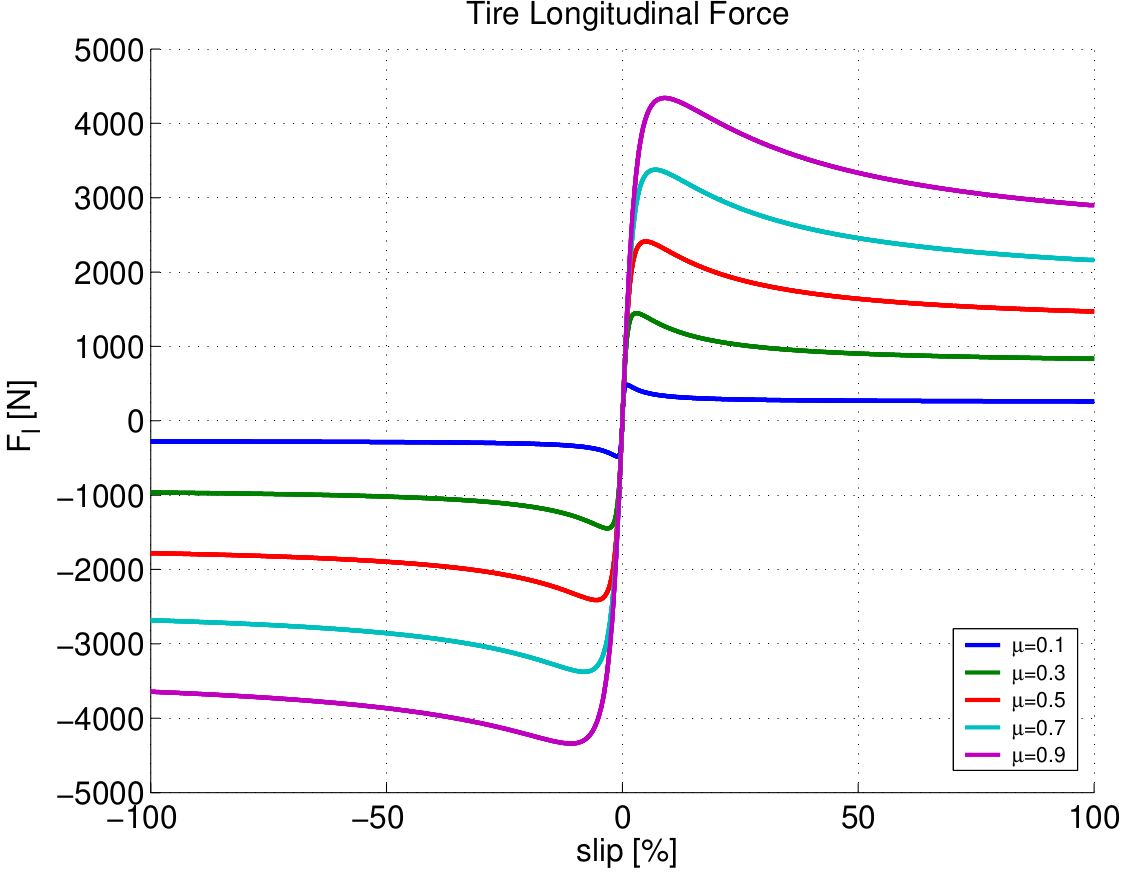
\includegraphics[width=\textwidth]{images/C14_5.png}
        \caption{Longitudinal force}
    \end{subfigure}
    \hfill
    \begin{subfigure}[b]{0.46\textwidth}
        \centering
        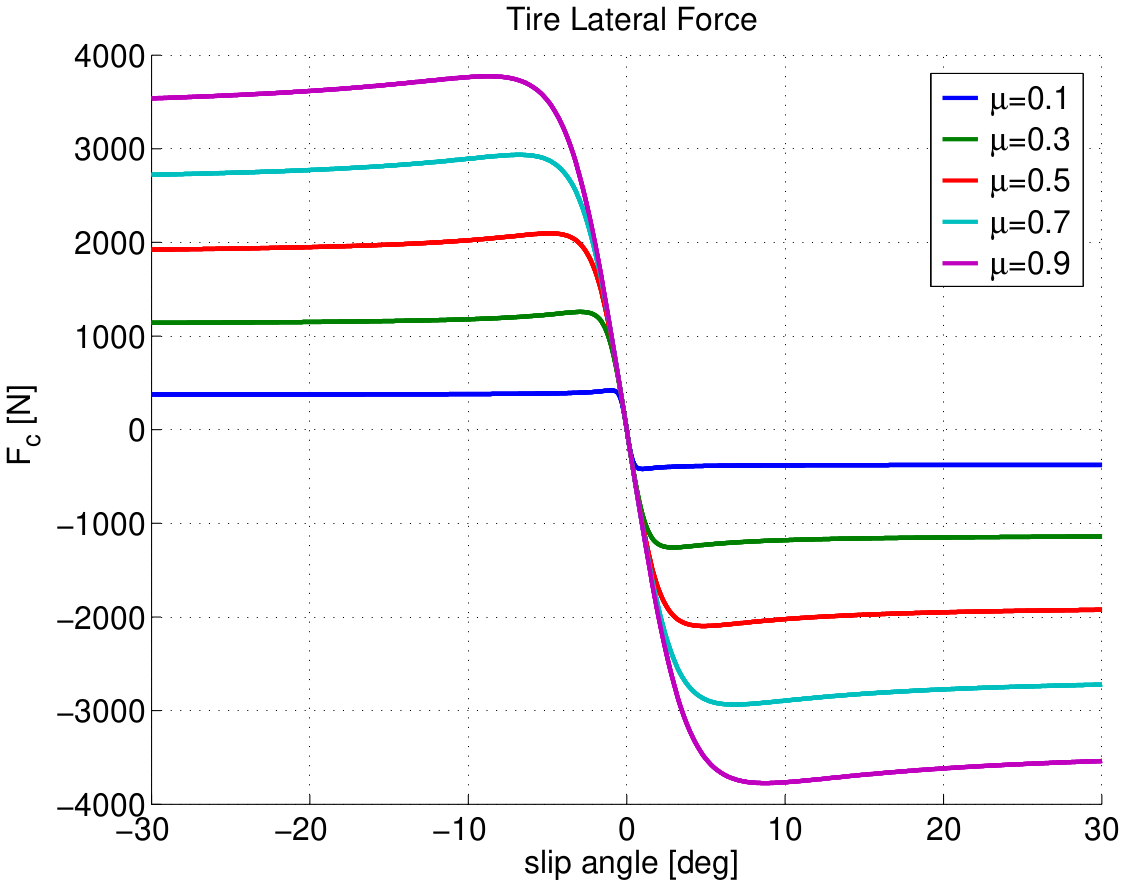
\includegraphics[width=\textwidth]{images/C14_6.png}
        \caption{Lateral force}
    \end{subfigure}
    \caption{Tire forces in pure driving/braking and pure cornering, for different values of $\mu$}
    \label{fig:tire-pure}
\end{figure}

\begin{infobox}[Sign conventions in the plots]
The plots use different sign conventions from the formulas above. In the longitudinal plot a positive slip gives a positive (traction) force, while $\lambda$ as defined above is positive in braking. In the lateral plot a positive slip angle gives a negative force, while the linear model below uses $F_y = C_y\,\alpha$. The shape of the curves does not change: only the sign of the axes does.
\end{infobox}

These curves describe pure driving/braking and pure cornering. In \textbf{combined} manoeuvres the two forces interact, as shown in Figure~\ref{fig:tire-combined}: the larger the slip angle, the lower the longitudinal force available at small slip, and vice versa. The tire has a limited amount of grip to share between the two directions.

\begin{figure}[H]
    \centering
    \begin{subfigure}[b]{0.46\textwidth}
        \centering
        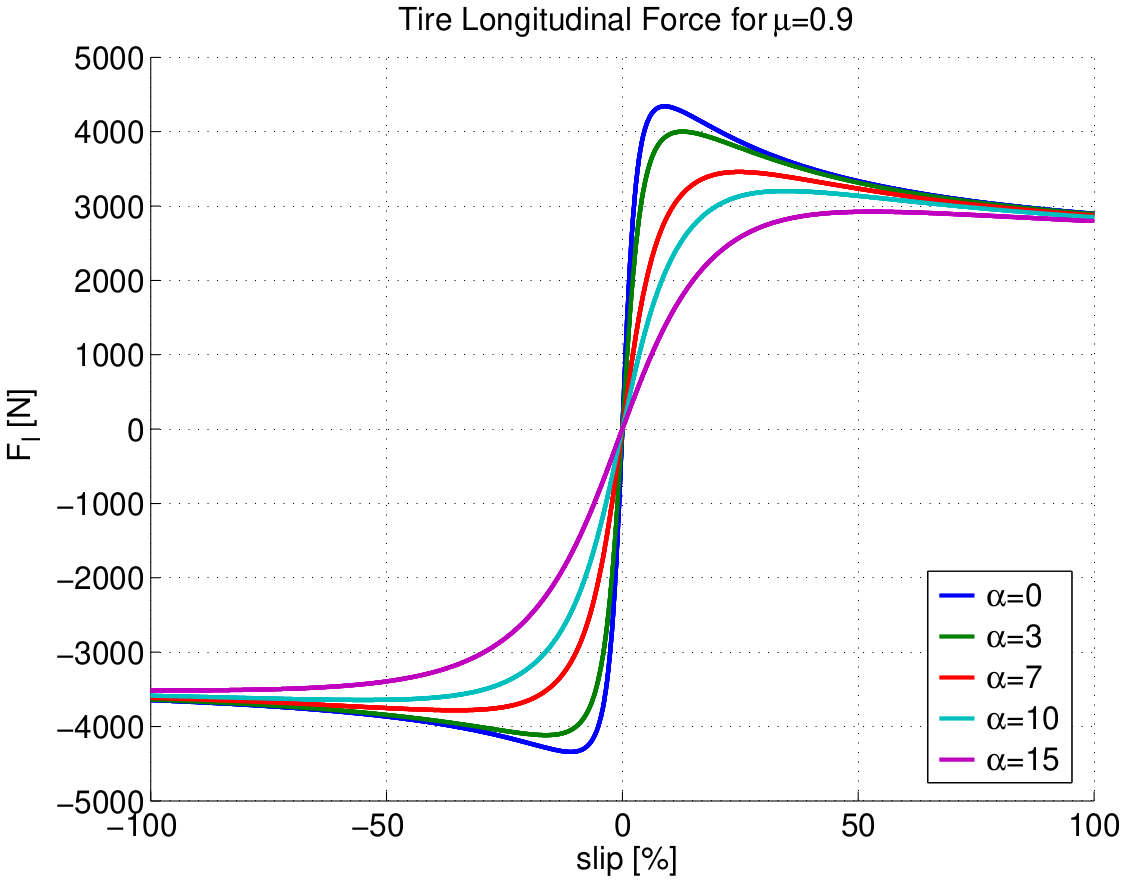
\includegraphics[width=\textwidth]{images/C14_7.png}
        \caption{Longitudinal force for different $\alpha$}
    \end{subfigure}
    \hfill
    \begin{subfigure}[b]{0.46\textwidth}
        \centering
        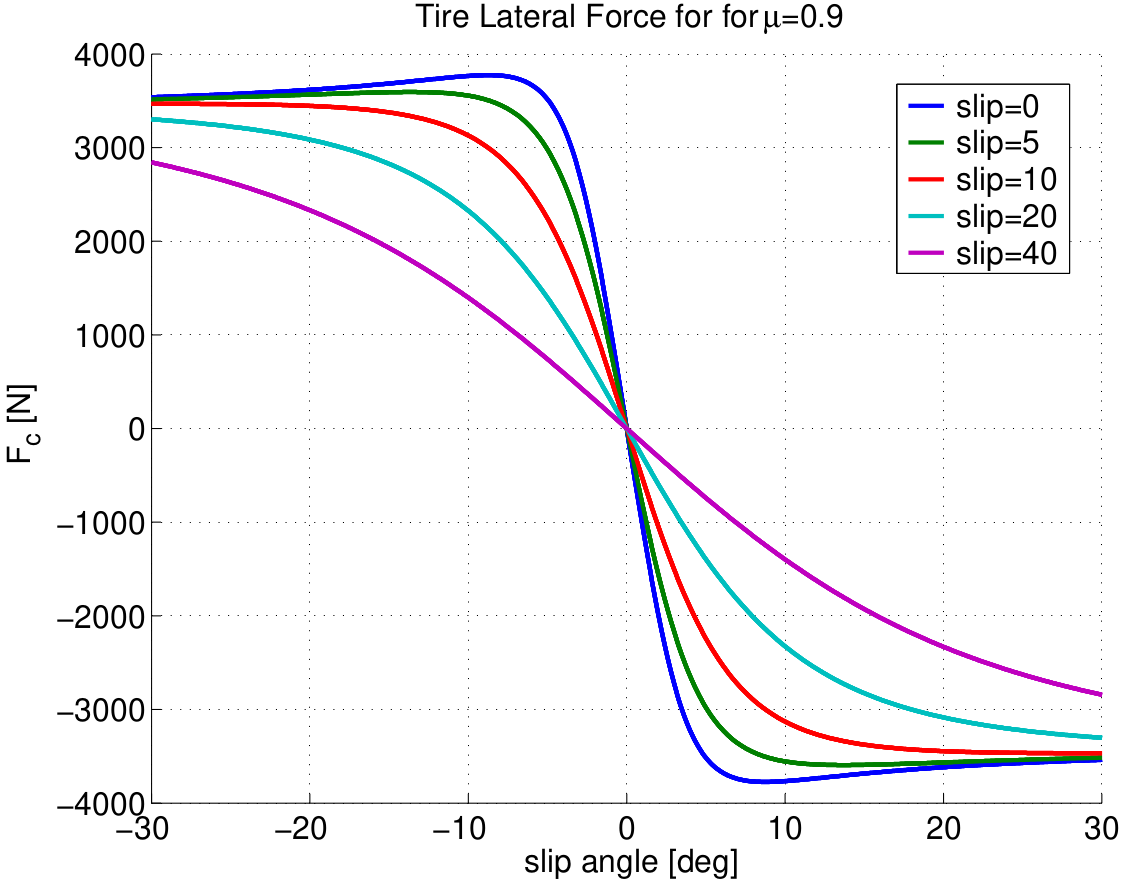
\includegraphics[width=\textwidth]{images/C14_8.png}
        \caption{Lateral force for different slip values}
    \end{subfigure}
    \caption{Tire forces in combined driving/braking and cornering, with $\mu = 0.9$}
    \label{fig:tire-combined}
\end{figure}

The physical modeling of tire forces can be very involved. Useful physical models exist (\textbf{Brush} model, \textbf{LuGre} friction model, \textbf{Dugoff}'s model), but the most widespread one is the semi-empirical \textbf{Pacejka} model.

\subsubsection{The Magic Formula}
The Pacejka tire model uses functions that are ``shaped'' to resemble the tire forces:
\[
Y(X) = D \sin\!\Big(C \arctan\big(B X - E\,(B X - \arctan(B X))\big)\Big)
\]
Here $Y$ is the generated longitudinal or lateral force, and $X$ is the slip ratio or the tire slip angle. The four parameters shape the curve and are \textbf{fitted on experimental data}:
\begin{compactitemize}
    \item $D$ is the \textbf{peak factor}, the maximum value of $Y$;
    \item $C$ is the \textbf{shape factor}, which sets the sharpness of the curve;
    \item $B$ is the \textbf{stiffness factor}, which sets how steep the curve is;
    \item $E$ is the \textbf{curvature factor}, which modifies the curvature near the peak.
\end{compactitemize}

\begin{figure}[H]
    \centering
    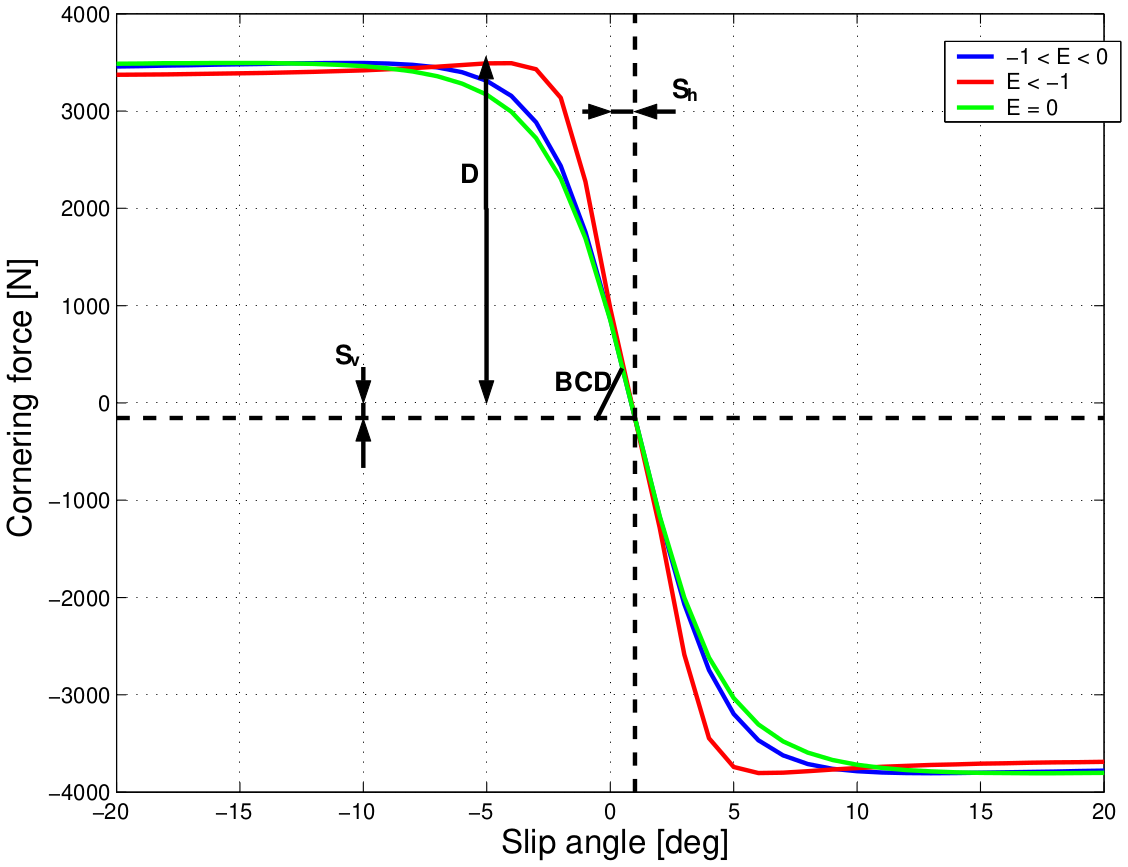
\includegraphics[width=0.52\textwidth]{images/C14_9.png}
    \caption{Magic Formula: peak $D$, slope $BCD$ at the origin and effect of $E$ ($S_h$ and $S_v$ are horizontal and vertical offsets of the curve)}
\end{figure}

\subsubsection{Linear tire model}
For small slip angles the force can be modeled in the linear region of the tire, using the \textbf{cornering stiffness} $C_y$:
\[
F_y = C_y\, \alpha
\]
\[
C_y = B\, C\, D
\]
The value of $C_y$ is the slope of the Magic Formula at the origin. Near $X = 0$ the argument of the sine is small, and the formula reduces to $Y \approx D\,C\,B\,X$. This assumption is valid \textbf{only for small slip angles}, as Figure~\ref{fig:linear-tire} shows.

\begin{figure}[H]
    \centering
    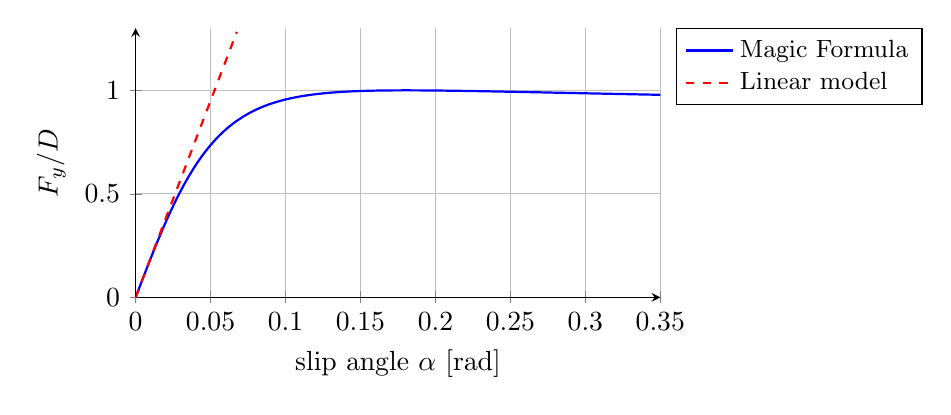
\begin{tikzpicture}
    \begin{axis}[
        width=0.68\textwidth, height=5cm,
        axis lines=left, grid=major,
        xlabel={slip angle $\alpha$ [rad]}, ylabel={$F_y / D$},
        xmin=0, xmax=0.35, ymin=0, ymax=1.3,
        xtick={0,0.05,0.1,0.15,0.2,0.25,0.3,0.35}, scaled x ticks=false,
        xticklabel style={/pgf/number format/fixed},
        samples=120, legend pos=outer north east, legend cell align=left,
        legend style={font=\small}]
        \addplot[blue, thick, domain=0:0.35] {sin(1.9*atan(10*x - 0.97*(10*x - rad(atan(10*x)))))};
        \addlegendentry{Magic Formula}
        \addplot[red, dashed, thick, domain=0:0.0675] {19*x};
        \addlegendentry{Linear model}
    \end{axis}
    \end{tikzpicture}
    \caption{Linear tire model and Magic Formula, with $B = 10$, $C = 1.9$, $E = 0.97$}
    \label{fig:linear-tire}
\end{figure}

\subsection{Longitudinal vehicle dynamics}
Figure~\ref{fig:longitudinal} shows the forces acting on a vehicle on a road with grade $\theta$. The figure calls this angle $\alpha$, but we use $\theta$ because $\alpha$ already denotes the slip angle.

\begin{figure}[H]
    \centering
    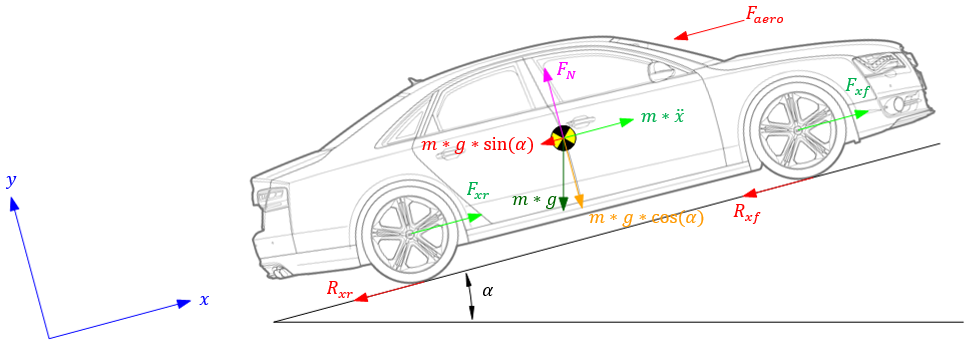
\includegraphics[width=0.7\textwidth]{images/C14_10.png}
    \caption{Forces acting on a vehicle along the longitudinal direction}
    \label{fig:longitudinal}
\end{figure}

Newton's law along the longitudinal axis of the vehicle gives:
\[
m\,\ddot x = F_{xf} + F_{xr} - F_{aero} - R_{xf} - R_{xr} - m\,g \sin\theta
\]
where $F_{xf}, F_{xr}$ are the front and rear longitudinal tire forces, $F_{aero}$ is the air drag and $R_{xf}, R_{xr}$ are the rolling resistance forces. For some applications of this course it can be simplified to:
\[
m\,\ddot x = F_x
\]

\subsubsection{Vertical forces}
The \textbf{vertical load}, or normal load, is the weight supported by each axle or wheel. The \textbf{vertical force} is any force acting vertically on the vehicle, and it is made of the static vertical load, the aerodynamic effects (lift or downforce) and the forces due to the suspensions. The total static load is:
\[
F_N = m\,g
\]
and it is split between the front and rear axles according to the position of the CoG:
\[
F_{Nf} = \frac{l_r}{l_{wb}}\, F_N
\]
\[
F_{Nr} = \frac{l_f}{l_{wb}}\, F_N
\]
These expressions come from the balance of moments around each axle. The closer the CoG is to an axle, the larger the load on that axle.

The vertical load can be included explicitly in the Magic Formula. For the rear lateral force:
\[
F_{yr}(\alpha) = F_{Nr}\, D \sin\!\Big(C \arctan\big(B\alpha - E\,(B\alpha - \arctan(B\alpha))\big)\Big)
\]
In this form $D$ is dimensionless, and the peak force is $F_{Nr}\,D$.

\subsubsection{Rolling resistance}
The \textbf{rolling resistance} opposes the motion of the vehicle on the road:
\[
R_x = C_r\, W
\]
where $R_x$ is the rolling resistance force (N), $W$ is the normal load on the wheel and $C_r$ is the rolling resistance coefficient, which depends on several characteristics such as the tire material, pressure and temperature. A second model also considers the dependency on speed:
\[
R_x = C_r\, W + K_v\, V
\]
where $K_v$ is a velocity-dependent rolling resistance coefficient and $V$ is the vehicle speed.

\subsubsection{Engine}
The force generated by the engine at the wheels is:
\[
F_e = \frac{T_{wheel}}{r_{wheel}}
\]
\[
T_{wheel} = T_{engine}\, \tau_{gear}\, \eta_{trans}
\]
where $T_{wheel}$ is the torque transmitted to the wheels through a transmission with gear ratio $\tau_{gear}$ and efficiency $\eta_{trans}$, and $r_{wheel}$ is the effective radius of the wheel.

For \textbf{electric motors} the torque is proportional to the current:
\[
T = k_t\, I
\]
where $k_t$ is the torque constant (Nm/A) and $I$ is the current supplied to the motor (A).

For \textbf{combustion engines} a simple model is:
\[
T_{engine} = T_{max} \left(1 - \left(\frac{\omega_{engine}}{\omega_{max}}\right)^{2}\right)
\]
where $T_{max}$ is the peak torque and $\omega_{engine}$ is the engine speed (rad/s). In this formula the torque equals $T_{max}$ at $\omega_{engine} = 0$ and goes to zero at $\omega_{engine} = \omega_{max}$, so $\omega_{max}$ is the maximum engine speed.

\begin{figure}[H]
    \centering
    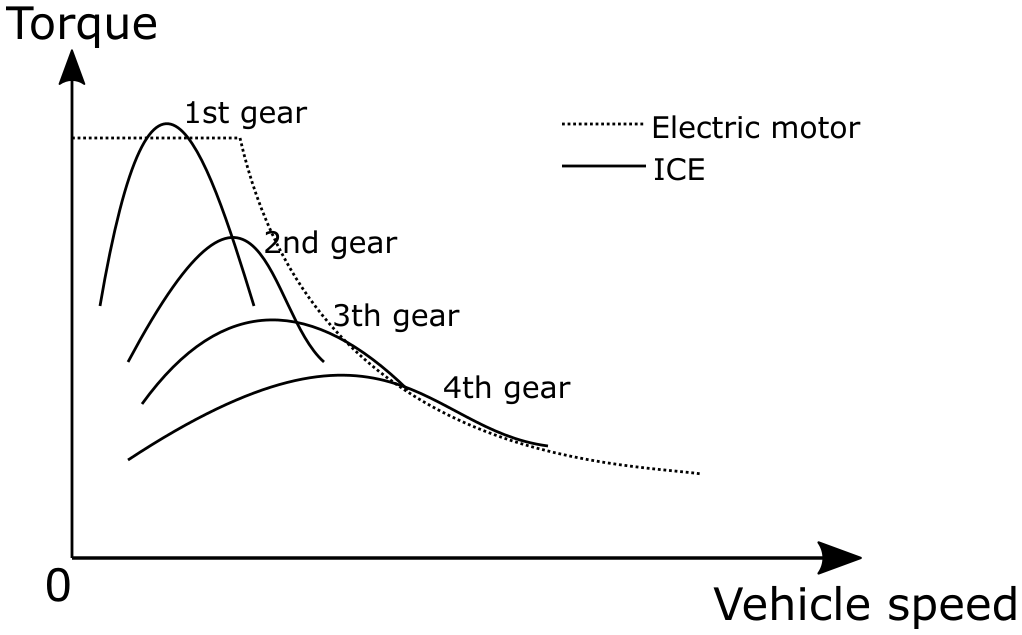
\includegraphics[width=0.36\textwidth]{images/C14_11.png}
    \caption{Torque as a function of vehicle speed: electric motor and combustion engine (ICE) with four gears}
\end{figure}

\subsubsection{Brakes}
A simplified model of the \textbf{brake force} is a function of the brake pedal input $B$:
\[
F_{br} = C_{br}\, B
\]
where $C_{br}$ is the maximum brake force at full brake input, usually estimated from the maximum brake pressure and the brake pad area, and $0 \le B \le 1$ is the normalized pedal input, i.e.\ the fraction of the maximum brake pressure applied. This $B$ has nothing to do with the stiffness factor of the Magic Formula.

\subsubsection{Aerodynamics}
The \textbf{drag force} is the resistance caused by the airflow interacting with the surface of the vehicle:
\[
F_{aero} = \frac{1}{2}\, \rho\, C_d\, S\, v^2
\]
where $\rho$ is the air density (kg/m$^3$), $C_d$ is the drag coefficient, $S$ is the frontal area of the vehicle (m$^2$) and $v$ is the vehicle speed (m/s). Drag has a great impact on fuel efficiency and on performance, for example on the top speed.

\begin{examplebox}[Why drag limits the top speed]
The power needed to overcome drag is $P = F_{aero}\, v$, so it grows with $v^3$. With $\rho = 1.2\,\mathrm{kg/m^3}$, $C_d = 0.3$ and $S = 2.2\,\mathrm{m^2}$:
\begin{center}
\begin{tabular}{c|c|c}
$v$ & $F_{aero}$ & $P$ \\ \hline
130 km/h & 517 N & 18.7 kW \\
260 km/h & 2066 N & 149 kW
\end{tabular}
\end{center}
Doubling the speed requires four times the force and eight times the power.
\end{examplebox}
